\section{Auswertung}
\label{sec:Auswertung}
Die in \autoref{sec:Auswertung} gezeigten Grafiken und Rechnungen sind mithilfe der Python-Bibliotheken Matplotlib \cite{matplotlib}, Scipy \cite{scipy} und Numpy \cite{numpy}
erstellt worden.


\begin{table}[H]
  \centering
  \caption{}
  \begin{tabular}{S[table-format=3] S[table-format=2(2)]}
      \toprule
      {$t\,/\symup{s}$} & {$N$} \\
      \midrule

      \bottomrule
  \end{tabular}
  \begin{tabular}{S[table-format=3] S[table-format=2(2)]}
      \toprule
      {$t\,/\symup{s}$} & {$N$} \\
      \midrule
      
      \bottomrule
  \end{tabular}
  \label{tab:}
\end{table}
%Plots und Bilder
%\begin{figure}[H]
%  \includegraphics[width=\linewidth]{plots/.pdf}
%  \caption{}
%  \label{fig:}
%\end{figure}


\subsection{Überprüfung der Stabilitätsbedingung}
Die Stabilitätsbedingung beschrieben in Gleichung (ref) beschreibt den Bereich der Resonatorlänge des HeNe LASERs in dem der LASER Strahl nicht divergiert. 
Für die Verwendeten Resonatoren, aus Konvex Konvex und Plan Konvex Spiegelaufbauten ergeben sich mit einem Krümmungsradius von $r = \SI{1400}{mm}$ für die Konvexen spiegel die Stabilitätsgleichungen
\begin{align}
  \left(g_1 \cdot g_2\right)_{\text{KK}} &= \left( 1 - \frac{L}{1400} \right)^2 \\
  \left(g_1 \cdot g_2\right)_{\text{PK}} &= 1 \cdot \left( 1 - \frac{L}{1400} \right) \, .
\end{align}
Diese Erfüllen die Stabilitätsbedingung für $0 \leq L \leq 2800 \, \, \mathrm{mm}$ für den Bikonvexen Resonator und $0 \leq L \leq 1400 \, \, \mathrm{mm}$ für den Plan Konvexen Resonator.
\\
\\
evtl theorie plot 
\\
\\
In Abbildung (ref) sind dabei die theoretischen Plots der Stabilitätsbedingung mit Eingezeichneten Grenzen zu sehen. 
\begin{table}[H]
  \centering
  \caption{Messwerte der LASER Leistung als Funktion der Resonatorlänge, KK Links und PK Rechts}
  \begin{tabular}{S[table-format=3] S[table-format=2(2)]}
      \toprule
      {$L$ / $\mathrm{cm}$} & {$P$ / $\mathrm{mW}$} \\
      \midrule
      45    &   6.99 \\
      50    &   6.33\\
      55    &   6.5\\
      60    &   4.89\\
      65    &   5.99\\
      70    &   4.23\\
      75    &   3.38\\
      80    &   5.17\\
      85    &   5.97\\
      90    &   6.4\\
      95    &   6.13\\
      100   &   4.23\\
      105   &   4.18\\
      110   &   4.87\\
      115   &   5.13\\
      120   &   4.65\\
      145   &   3.4\\
      \bottomrule
  \end{tabular}
  \begin{tabular}{S[table-format=3] S[table-format=2(2)]}
      \toprule
      {$L$ / $\mathrm{cm}$} & {$P$ / $\mathrm{mW}$} \\
      \midrule
      55.5 & 1.2\\
      70  & 0.57\\
      80 & 0.72\\
      90 & 2.14\\
      100 & 1.8\\
      110 & 0.7\\
      \\
      \\
      \\
      \\
      \\
      \\
      \\
      \\
      \\
      \\
      \\
      \bottomrule
  \end{tabular}
  \label{tab:1}
\end{table}
\noindent
In \autoref{tab:1} sind die Daten der Messreihe zur Verifizierung der Stabilitätsbedingung zu sehen. In diesen ist zu erkennen, dass der Bikonvexe Resonator auch bei Resonatorlängen über $\SI{1400}{mm}$ stabil Funktioniert. 
\begin{figure}[H]
  \centering
  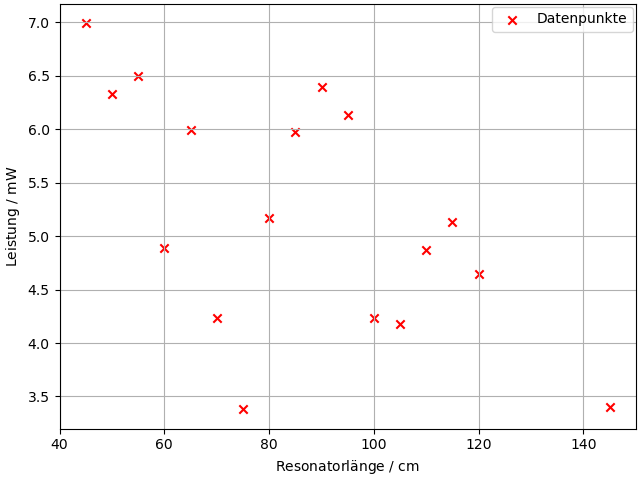
\includegraphics[width=0.6\linewidth]{plots/stab_bed_1.png}
  \caption{Leistung des LASERs als Funktion der Resonatorlänge}
  \label{fig:1}
\end{figure}
\noindent
Die Leistung des LASERs ist dabei unabhängig von der Länge des Resonators wie in \autoref{fig:1} gut zu erkennen ist.
\newpage
\subsection{Messung der Wellenlänge des LASERs}
\newpage
\subsection{Messung der Polarisationsrichtung des LASERs}
In \autoref{tab:2} sind die Messwerte der Messreihe für die Bestimmung der Polarisationsrichtung des LASERs zu sehen.
\begin{table}[H]
  \centering
  \caption{Messwerte der Leistung des LASERs als Funktion des Polarisationswinkels}
  \begin{tabular}{S[table-format=3] S[table-format=2(2)]}
      \toprule
      {Winkel $\Phi$ / $^\circ$} & {$P$ / $\mathrm{mW}$} \\
      \midrule
      0    &0.45 \\
      10   &0.96 \\
      20    &1.56 \\
      30    &2.15 \\
      40    &2.73 \\
      50    &3.13 \\
      60    &3.47 \\
      70    &3.58 \\
      80    &3.45 \\
      90    &3.07 \\
      100    &2.69 \\
      110    &2.06 \\
      120    &1.39 \\
      130    &0.82 \\
      140    &0.37 \\
      150    &0.1 \\
      160    &0.0 \\
      170    &0.13  \\
      \bottomrule
  \end{tabular}
  \begin{tabular}{S[table-format=3] S[table-format=2(2)]}
    \toprule
    {Winkel $\Phi$ / $^\circ$} & {$P$ / $\mathrm{mW}$} \\
    \midrule
    180    &0.45  \\
    190    &0.97 \\
    200    &1.54 \\
    210    &2.24 \\
    220    &2.77 \\
    230    &3.18 \\
    240    &3.5 \\
    250    &3.53 \\
    260    &3.37 \\
    270    &3.0 \\
    280    &2.66 \\
    290    &2.01 \\
    300    &1.39 \\
    310    &0.87 \\
    320    &0.37 \\
    330    &0.08 \\
    340    &0.0 \\
    350    &0.12 \\
    \bottomrule
  \end{tabular}
  \label{tab:2}
\end{table}
\noindent 
Diese sind nach Gleichung (ref) proportional zu $\text{cos}^2\left(\Phi\right)$, wobei die Funktion maximal wird wenn der Polarisationswinkel $\Phi_0$ erreicht ist. Dies ist durch eine Phasenverschiebung um diesen Winkel erreichbar, weswegen eine Funktion der Form 
\begin{equation}
  \label{eqn:1}
  P\left(\Phi\right) = I_0 \cdot \text{cos}^2\left(\Phi - \Phi_0\right)
\end{equation}
in die Daten gefittet wurde.
\begin{figure}[H]
  \centering
  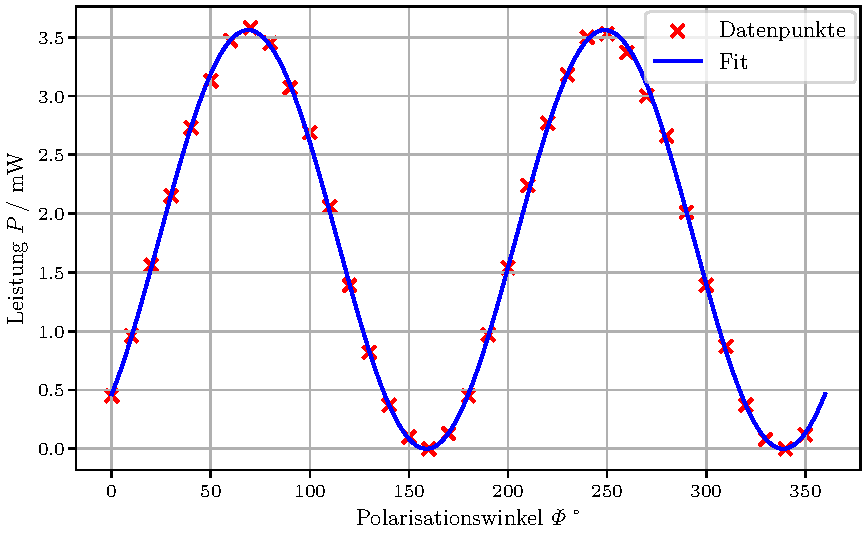
\includegraphics[width=0.7\linewidth]{plots/pol.pdf}
  \caption{Leistung des LASERs als Funktion des Polarisationswinkels}
  \label{fig:2}
\end{figure}
\noindent
In \autoref{fig:2} Sind die Daten in einem Scatter Plot aufgetragen und der zugehörige Fit der Funktion in \autoref{eqn:1} zu sehen.
Die Parameter der Gleichung lassen sich dabei auf 
\begin{align}
  \Phi_0 &= 68.834 \pm 0.018 \, \, ^\circ \\
  I_0 &= 3.56078 \pm 0.00009 \, \, \mathrm{mW}
\end{align}
wobei $I_0$ die Leistung des Lasers ohne Polarisationsfilter ist. 
\noindent
\newpage 
\subsection{Abhängigkeit der longitudinalen Resonatormoden von der Resonatorlänge}
\newpage